\documentclass{endm}
\usepackage{endmmacro}
\usepackage{graphicx}
\usepackage{amsmath}
\usepackage{caption}
\usepackage[brazilian,english]{babel}
\usepackage[utf8]{inputenc}
\usepackage[T1]{fontenc}
\usepackage{multirow}

% The following is enclosed to allow easy detection of differences in
% ascii coding.
% Upper-case    A B C D E F G H I J K L M N O P Q R S T U V W X Y Z
% Lower-case    a b c d e f g h i j k l m n o p q r s t u v w x y z
% Digits        0 1 2 3 4 5 6 7 8 9
% Exclamation   !           Double quote "          Hash (number) #
% Dollar        $           Percent      %          Ampersand     &
% Acute accent  '           Left paren   (          Right paren   )
% Asterisk      *           Plus         +          Comma         ,
% Minus         -           Point        .          Solidus       /
% Colon         :           Semicolon    ;          Less than     <
% Equals        =           Greater than >          Question mark ?
% At            @           Left bracket [          Backslash     \
% Right bracket ]           Circumflex   ^          Underscore    _
% Grave accent  `           Left brace   {          Vertical bar  |
% Right brace   }           Tilde        ~

\newcommand{\Nat}{{\mathbb N}}
\newcommand{\Real}{{\mathbb R}}
\def\lastname{Brito}

\begin{document}  

% DO NOT REMOVE: Creates space for Elsevier logo, ScienceDirect logo
% and ENDM logo
\begin{verbatim}\end{verbatim}\vspace{2.5cm}

\begin{frontmatter}

\title{The Set Packing Polytope: A Computational Study of Conflict Graphs and Aggressive Cut Separation}
\author{Samuel Souza Brito \and Haroldo Gambini Santos\thanksref{mailSamuelHaroldo}}
\address{{\small Departamento de Computação, Universidade Federal de Ouro Preto - UFOP}}
\author{Marcus Poggi\thanksref{mailPoggi}}
\address{{\small Dep. de Informática, Pontifícia Universidade Católica do Rio de Janeiro}}
\thanks[mailSamuelHaroldo]{Email: {\texttt{\normalshape \{samuelsouza,haroldo\}@iceb.ufop.br}}} 
\thanks[mailPoggi]{Email: {\texttt{\normalshape poggi@inf.puc-rio.br}}}  

\begin{abstract}
This work explores the fast creation of densely populated conflict graphs at the root node of the search tree for integer programs. We show that not only the Generalized Upper Bound (GUB) constraints are useful for the fast detection of cliques: these can also be quickly detected in less structured constraints in $O( n \log n )$. Routines for the aggressive separation and lifting of cliques and odd-holes are proposed. Improved bounds and a faster convergence to strong bounds were observed when comparing to the default separation routines found in the current version of the COmputation INfrastructure for Operations Research (COIN-OR) Branch and Cut solver.
\end{abstract}

\begin{keyword}
conflict graphs, integer programming, cutting planes, cliques, odd holes
\end{keyword}

\end{frontmatter}


\section{Introduction}\label{intro}

Conflict Graphs (CG) represent logical relations between binary variables: vertices represent variables and edges indicate that two variables cannot be set to specific values without violating one or more constraints. CGs are typically constructed using probing techniques\cite{Borndorfer1998} based on constraints analysis. On this work we propose techniques to speed up the creation of dense conflict graphs at the root node. Exact separation routines are employed to discover all violated cliques and odd holes, which are lifted in subsequent steps.

In Section \ref{seccgraph} we formally explain our approach to build conflict graphs as well as our strategy to speedup the detection of logical implications; in Section \ref{cut} we present the cut separation and lifting routines; in Section \ref{experiments} computational experiments are presented and finally, in Section \ref{conclusions} we conclude and discuss the results of this work.

\section{Conflict Graphs in Integer Programming}\label{seccgraph}

A conflict graph represents logical relations between binary variables. For two binary variables, we may discover four possible logical relations, using the notation of \cite{atamturk}: (i) $x = 1 \Rightarrow y = 1 \Longleftrightarrow x + (1 - y)  \leq 1$ ; (ii) $x=1 \Rightarrow y = 0 \Longleftrightarrow x + y \leq 1$; (iii) $x = 0 \Rightarrow y = 1 \Longleftrightarrow  (1 - x) + (1 - y) \leq 1$ and (iv) $x = 0 \Rightarrow y = 0 \Longleftrightarrow (1 - x) + y \leq 1$.

Given an Integer Program (IP), a conflict graph can be constructed using probing techniques based on feasibility considerations\cite{achterberg,atamturk}, checking the impact of fixing pairs of variables to different combinations of values. First, consider that each constraint $i \in \{1,\ldots,m\}$ can be written as $\displaystyle \sum_{j \in N} a_{ij}x_{j} \leq b_{i}$, where $N=\{1,\ldots,n\}$ is the index set of binary variables $x$, $a_{ij}$ is the coefficient for variable $x_{j}$ at constraint $i$ and $b_{i}$ is the right-hand side of constraint $i$. Suppose we are analyzing two particular variables $x_{\hat{j}}$ and $x_{\hat{k}}$ with respect to constraint $i$. Consider that these variables are assigned with values $u$ and $v$, respectively. Consider also that $N_{i}^{-} = \{j \in N : a_{ij} < 0\}$. Then, $\displaystyle
L_{i}^{x_{\hat{j}} = u,\, x_{\hat{k}} = v}=\sum_{j\in N_{i}^{-} \setminus \{\hat{j}, \hat{k}\}}a_{ij}+a_{i\hat{j}}u+a_{i\hat{k}}v $, is a lower bound for the value on the left-hand side  of the constraint $i$, considering the assignments $(x_{\hat{j}} =u,x_{\hat{k}}=v)$. If $L_{i}^{x_{\hat{j}} = u,\, x_{\hat{k}} = v} > b_{i}$, a conflict is detected for these assignments. 

Performing these steps considering each pair of variables in each constraint, leads to the creation of a conflict graph in $O(m \times n^2)$.  Nevertheless, for some constraint types a large number of conflicts can be quickly discovered. This is the case of the Generalized Upper Bound constraints ($\sum_{j\in N}x_j \leq 1$). The following subsection will describe additional cases where cliques in individual constraints can be quickly detected (i.e., faster than $O(n^2)$). The following notation will be used: $\tilde{a}_{ik}$ is the $k$-th smallest coefficient in constraint $i$ and $\acute{a}_{ik}$ indicates its index. Constants $n_i$ and $S_i^-$ denote the number of non-zero variables and the sum of all negative coefficients of constraint $i$, respectively. In the next paragraphs fast clique detection will be discussed for additional constraint structures. 

We describe two cases where large cliques of conflicting variables can be detected just by traversing constraints with  coefficients of variables sorted in non-decreasing order. Thus, conflicts in these constraints are discovered in $O( n \log n)$. At first, consider that at a given position $k$ the summation of negative coefficients excluding the pair of variables at positions $k$ and $k+1$ is: $\displaystyle D_{i}^{x_{\acute{a}_{ik}}, x_{\acute{a}_{ik+1}}} = S_i^- - min(0, \tilde{a}_{ik}) - min(0, \tilde{a}_{ik+1})$.  Thus, the lower bound for the LHS of constraint $i$ when variables with the $k-$th and $(k+1)-$th smallest coefficients are fixed at one is: $\displaystyle LHS_{i}^{x_{\acute{a}_{ik}} = 1, x_{\acute{a}_{ik+1}} = 1} = D_{i}^{x_{\acute{a}_{ik}}, x_{\acute{a}_{ik+1}}} + \tilde{a}_{ik} + \tilde{a}_{ik+1}$.

Since $LHS_{i}^{x_{\acute{a}_{ik}} = 1, x_{\acute{a}_{ik+1}} = 1}$ is monotonically non-decreasing as $k$ increases, if $LHS_{i}^{x_{\acute{a}_{ik}} = 1, x_{\acute{a}_{ik+1}} = 1} > b_{i}$, then there is a clique involving the activation of all variables from position $k$ until position $n_i$. Moreover, we can discard the existence of such cliques by checking if $LHS_{i}^{x_{\acute{a}_{in_i-1}} = 1, x_{\acute{a}_{in_i}} = 1} \leq b_i$. Analogously, cliques involving complementary variables from positions $n_i$ until $k$ can be obtained or discarded checking the limit incurred from positions $k$ and $k-1$  $LHS_{i}^{x_{\acute{a}_{ik}} = 0, x_{\acute{a}_{ik-1}} = 0} = D_{i}^{x_{\acute{a}_{ik}}, x_{\acute{a}_{ik-1}}} $. For variables which are not involved in these easy to compute cliques a pairwise analysis is performed for each constraint. 

\begin{figure}
{\small

\begin{minipage}[b]{.5\textwidth}
 \[ \mathcal{P} = \left\{
\begin{array}{lr}
x_1+x_2+x_3 & \geq 2 \\
-2x_{1}+3x_{2}+4x_{3}+5x_{4} & \leq 4 \\
x_{1},\ldots,x_{4}\in\{0,1\}
\end{array}
\right. \]
\end{minipage}
\begin{minipage}{.5\textwidth}
	\centering
	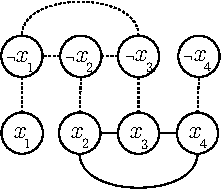
\includegraphics[width=3.0cm]{cGraph.pdf}
\end{minipage}
}
\caption{A binary program and its conflict graph}\label{graph}
\end{figure}

As an illustrative example, Figure \ref{graph} shows the conflict graph for a binary program $\mathcal{P}$, where $\neg x_i$ represents the complement (or deactivation) of variable $x_i$. Normal lines indicate conflict between original variables and dashed lines indicate conflict between complimentary variables.

\section{Cutting Planes}\label{cut}

Linear programming relaxations can be significantly strengthened by the inclusion of inequalities derived from the set packing polytope (SPP) \cite {Padberg1973}. A clique inequality for a set $C$ of conflicting variables has the form $\sum_{j\in C}x_{j} \leq 1$ and an odd-hole inequality with conflicting variables $C$ can be defined as: $\sum_{j\in C}x_{j} \leq \lfloor \frac{|C|}{2}\rfloor$. Considering generic clique separation routines, the most common ones are the star clique and the row clique method \cite{Borndorfer1998}, which are used in the current version of the COIN-OR\cite{LougeeHeimer2003} Cut Generation Library (CGL).  

\begin{figure}	
	\begin{minipage}[h]{.5\textwidth}
		\begin{center}
			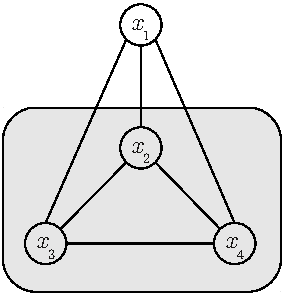
\includegraphics[width=0.5\textwidth]{clique.pdf}
		\end{center}
	\end{minipage}
	\begin{minipage}[h]{.5\textwidth}
		\begin{center}
			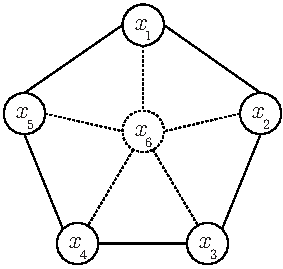
\includegraphics[width=0.5\textwidth]{oddHole.pdf}
		\end{center}
	\end{minipage}
	\caption{Example of a $k_{3}$ which could be lifted to a $k_{4}$    and an odd hole and its possible extension to a wheel} \label{figLiftings}
\end{figure}

Our proposed clique separation routine has two main components: (i) a module to separate all violated cliques in the conflict subgraph induced by the fractional variables and (ii) a lifting module which extends generated cliques considering the original conflict graph. The clique separation module was implemented using an improved version of the Bron-Kerbosch algorithm \cite{Bron1973}. This version implements an optimized pivoting rule \cite{Brito2011} to speed up the discovery of maximal cliques with large weight.  We also lift all generated inequalities as presented in Figure \ref{figLiftings}, using greedy heuristics, giving higher priority to inactive variables with the smallest reduced cost. Lifted clique inequalities have the same structure: only ones in the left-hand side. A lifted Odd-hole for variables $C$ and a wheel center $W$ can be written as $\displaystyle 	\sum_{j \in W} \lfloor \frac{|C|}{2} \rfloor x_{j} + \sum_{j \in C} x_{j} \leq \lfloor \frac{|C|}{2} \rfloor$.

\begin{figure}
\begin{center}
\label{figOH}
\end{center}
\end{figure}

\section{Experimental Results}\label{experiments}

Our code was written using the open source COIN-OR CLP libraries to solve linear programs and the CGL library was used to compare with our cut generation routines. All experiments ran in a computer with an Intel Core i7 3.6GHz processor and 32GB of RAM.

The first set of instances is the benchmark set of from MIPLIB 3, 2003 and 2010 \cite{miplib}. The second set of instances (INRC) comes from an IP formulation  used to solve the Nurse Rostering Problem \cite{Santos2014} of the International Nurse Rostering Competition. Finally, the Telebus set consists in set partitioning problems from \cite{Borndorfer1998}. After removing infeasible instances and instances where neither our code or CGL found violated inequalities the remaining instances in each set were 21, 40 and 14, respectively. Characteristics of each problem set are presented in Table \ref{tab:inst}: columns ($n$), rows ($m$), non-zeros ($nz$) and the number of edges in conflict graphs (CG) inferred from all pairwise, individual constraint based evaluation is also shown. ($\underline{v}$,$\overline{v}$,$\tilde{v}$) indicates minimum, maximum and average values. Finally, the total processing time obtained with pairwise detection (PD) and with our algorithm (FCG). 

\begin{table}[h]
\scriptsize
\caption{Characteristics of instance sets and their conflict graphs.}\label{tab:inst}
\begin{center}
\begin{tabular}{|l|c|c|c|c|r|r|}
\hline 
\multirow{2}{0.8cm}{Inst. Set} & \multicolumn{3}{c|}{{Problem Sizes ($\times10^{3}$)}} & {CG ($\times10^{6}$)} & \multicolumn{2}{c|}{{Time (s)}}\tabularnewline
\cline{2-7} 
 & {$\underline{n}$/$\overline{n}$/$\tilde{n}$} & {$\underline{m}$/$\overline{m}$/$\tilde{m}$} & {$\underline{nz}$/$\overline{nz}$/$\tilde{nz}$} & {$|\underline{E}|$/$|\overline{E}|$/$\tilde{|E|}$} & \multicolumn{1}{c|}{PD} & \multicolumn{1}{c|}{FCG}\tabularnewline
\hline 
\hline 
\texttt{MIPLIB} & {0.1/164.6/13.7} & {0.1/624.2/32.1} & {0.7/27678.7/515.9} & {0/11.4/0.4} & {198.8} & {17.5}\tabularnewline
\hline 
\texttt{INRC} & {9.8/63.6/29.7} & {3/29.2/11.7} & {201.1/1068.1/534.8} & {2.5/12.8/6.5} & {713.0} & {496.3}\tabularnewline
\hline 
\texttt{Telebus} & {1.1/146.7/33.7} & {0.3/1.8/1} & {1.4/545.3/135.6} & {0.1/1935.5/80} & {14734.6} & {540.2}\tabularnewline
\hline 
\end{tabular}
\end{center}
\end{table}

Figure \ref{figExperiments} shows the average gap closed improvement for each instance set where cgl and our separation routines npsep and lnpsep (lifted) are compared. While remarkable improvements were obtained in the INRC instances, which have a large number of dense set partitioning and packing constraints, a modest improvement occurred in MIPLIB instances, the average lower bound improved from 51.06, obtained with CGL, to 53.39, obtained with lnpsep within the time limit imposed. We did not included the Telebus results because all strategies performed equally well on these instances.

\begin{figure}	
	\begin{minipage}[h]{.5\textwidth}
		\begin{center}
			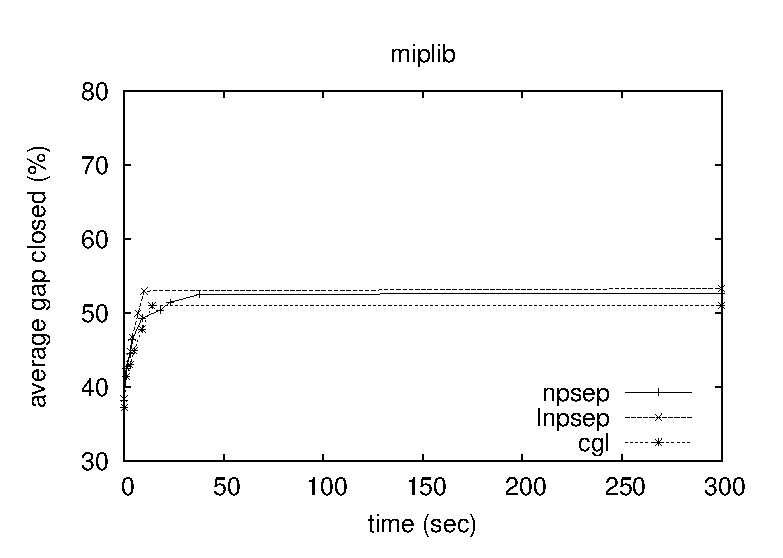
\includegraphics[width=1\textwidth]{miplib.eps}
		\end{center}
	\end{minipage}
	\begin{minipage}[h]{.5\textwidth}
		\begin{center}
			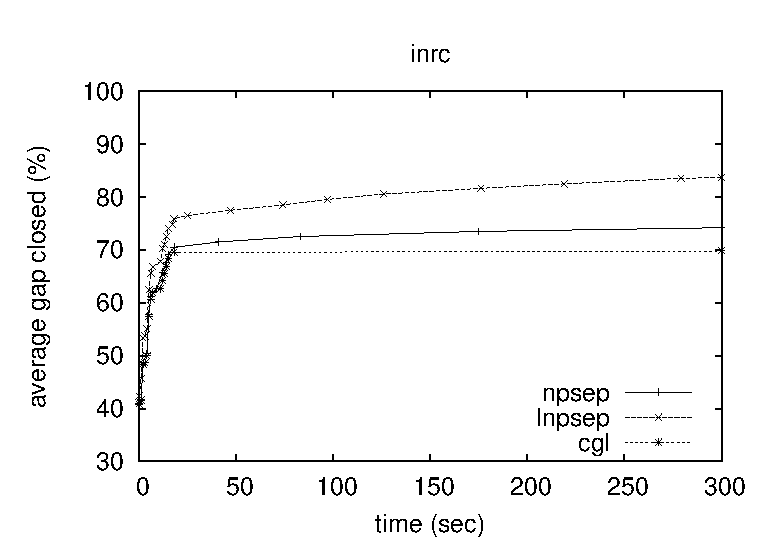
\includegraphics[width=1\textwidth]{nurse.eps}
		\end{center}
	\end{minipage}
	\caption{Dual bound improvement using npsep, lnpsep and cgl cuts.}
	\label{figExperiments}
\end{figure}

\section{Conclusions}\label{conclusions}

We developed an approach for fast creation of densely CGs using the detection of cliques in less structured constraints. A speedup of up to 30 times was obtained in the overall time to create an initial conflict graph. We also proposed and implemented an exact cut separation procedure. Experiments show that our cut generator can produce significantly better dual bounds than CGL, specially in restricted execution times.

\bibliographystyle{endm}
\bibliography{references}

\end{document}
